\documentclass{article}



\usepackage{fullpage}
\usepackage{nopageno}
\usepackage{amsmath}
\usepackage{amsfonts}
\usepackage{graphicx}
\usepackage{framed}
\usepackage{xcolor}

\definecolor{dark_red}{rgb}{0.5,0.0,0.0}
\definecolor{dark_green}{rgb}{0.0,0.5,0.0}
\definecolor{dark_blue}{rgb}{0.0,0.0,0.5}

\newcommand{\dr}[1]{\textcolor{dark_red}{#1}}
\newcommand{\dg}[1]{\textcolor{dark_green}{#1}}
\newcommand{\db}[1]{\textcolor{dark_blue}{#1}}


\begin{document}

{\bf In the discussions that will follow, an arbitrary triangle (not necessarily right angled) will have the side lengths denoted \(A\), \(B\), and \(C\). The angles opposite sides \(A\), \(B\), and \(C\) will be named \(\theta_A\), \(\theta_B\), and \(\theta_C\) respectively.} 

\section*{Triangle angles sum to $180^\circ$}

\begin{tabular}{cc}
\parbox{0.7\textwidth}{
The angles of a triangle sum to \(180^\circ\). In the image to the right, 
%the sides are labeled \(A\), \(B\), and \(C\), and the angles opposite \(A\), \(B\), and \(C\) are respectively named \(\theta_A\), \(\theta_B\), and \(\theta_C\). 
a dashed line is drawn parallel to side \(C\) through the vertex opposite side \(C\). By translating the angles \(\theta_A\) and \(\theta_B\) onto this dashed line, it can easily be seen that \(\theta_A + \theta_B + \theta_C = 180^\circ\).
} & \parbox{0.3\textwidth}{
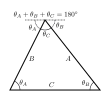
\includegraphics[width = 0.3\textwidth]{triangle_angles_sum_to_180}
}
\end{tabular}

\textbf{Examples:}
\begin{itemize}
\item If \(\theta_A = 34^\circ\), and \(\theta_B = 72^\circ\), then \(\theta_C = 180^\circ - \theta_A - \theta_B = 74^\circ\).   
\item If \(\theta_B = 47^\circ\), and \(\theta_C = 74^\circ\), then \(\theta_A = 180^\circ - \theta_B - \theta_C = 59^\circ\).
\item If \(\theta_A = 23^\circ\), and \(\theta_C = 52^\circ\), then \(\theta_B = 180^\circ - \theta_A - \theta_C = 105^\circ\).
\item If \(\theta_A = 123^\circ\), and \(\theta_B = 25^\circ\), then \(\theta_C = 180^\circ - \theta_A - \theta_B = 32^\circ\).
\item If \(\theta_B = \pi/4\), and \(\theta_C = \pi/3\), then \(\theta_A = \pi - \theta_B - \theta_C = 5\pi/12\). \\
Alternately, one can compute: \(\theta_A = 180^\circ - \theta_B - \theta_C = 180^\circ - 45^\circ - 60^\circ = 75^\circ\).
\item If \(\theta_A = 30^\circ\), and \(\theta_C = \pi/3\), then \(\theta_B = \pi - \theta_A - \theta_C = \pi - \pi/6 - \pi/3 = \pi/2\). \\
Alternately, one can compute: \(\theta_B = 180^\circ - \theta_A - \theta_C = 180^\circ - 30^\circ - 60^\circ = 90^\circ\).
\end{itemize}



\section*{The Sine Law}  

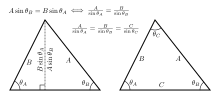
\includegraphics[width = \textwidth]{sine_law_for_triangles}

Given an arbitrary triangle, the length \(h\) of the altitude that descends from the vertex with angle \(\theta_C\) and is perpendicular to side \(C\), can be computed in two different ways, as seen in the image above. The altitude splits the triangle into two right triangles that share the altitude \(h\) as their opposites. The right triangle with angle \(\theta_A\) has \(B\) as its hypotenuse, while the right triangle with angle \(\theta_B\) has \(A\) as its hypotenuse. The triangle with angle \(\theta_A\) computes \(h = B\sin\theta_A\), while the triangle with angle \(\theta_B\) computes \(h = A\sin\theta_B\). Hence \(A\sin\theta_B = B\sin\theta_A\) which is equivalent to \(\frac{A}{\sin\theta_A} = \frac{B}{\sin\theta_B}\). By replacing \(A\) and \(\theta_A\) with \(C\) and \(\theta_C\) respectively, exactly analogous reasoning gives: \(\frac{C}{\sin\theta_C} = \frac{B}{\sin\theta_B}\). Combining these two equations gives:
\[\frac{A}{\sin\theta_A} = \frac{B}{\sin\theta_B} = \frac{C}{\sin\theta_C}\]
This equation is known as the {\bf Sine Law}.



\section*{The Cosine Law}

\begin{tabular}{cc}
\parbox{0.5\textwidth}{
Given the triangle on the right, the altitude descending from the top vertex splits the triangle into two right triangles. The named angle of the left hand triangle is \(\theta_C\) and the hypotenuse is \(B\). The adjacent is \(B\cos\theta_C\), and the opposite is \(B\sin\theta_C\). The orthogonal sides of the right hand triangle are \(A - B\cos\theta_C\) and \(B\sin\theta_C\), and the hypotenuse is \(C\). The Pythagorean theorem gives:
\begin{align*}
& C^2 = (A - B\cos\theta_C)^2 + (B\sin\theta_C)^2 \\
\iff & C^2 = (A^2 - 2AB\cos\theta_C + B^2\cos^2\theta_C) + B^2\sin^2\theta_C \\
\iff & C^2 = A^2 - 2AB\cos\theta_C + B^2(\cos^2\theta_C + \sin^2\theta_C) \\
\iff & C^2 = A^2 + B^2 - 2AB\cos\theta_C
\end{align*}
} & \parbox{0.5\textwidth}{
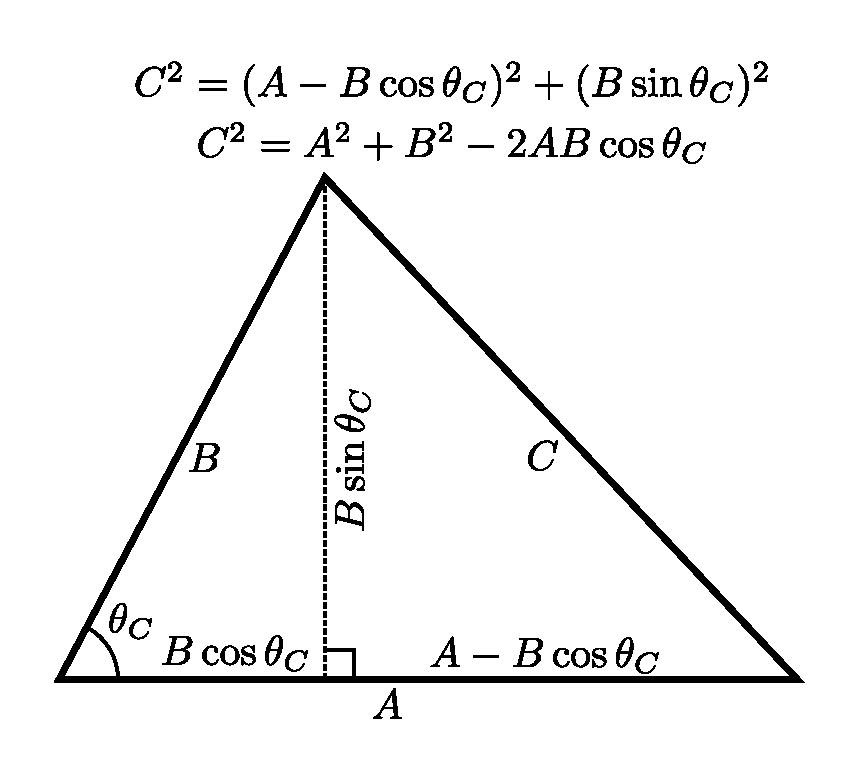
\includegraphics[width = 0.5\textwidth]{cosine_law_for_triangles}
}
\end{tabular}

Therefore:
\[C^2 = A^2 + B^2 - 2AB\cos\theta_C\]
This equation is known as the {\bf Cosine Law}. It should be noted that the cosine law holds for the other choices of sides and angles, provided that the angle is between the two sides:
\begin{itemize}
\item \(A^2 = B^2 + C^2 - 2BC\cos\theta_A\)
\item \(B^2 = A^2 + C^2 - 2AC\cos\theta_B\)
\item \(C^2 = A^2 + B^2 - 2AB\cos\theta_C\)
\end{itemize}




\section*{Solving triangles with the sine and cosine laws}

``Solving a triangle" refers to find all unknown sides and angles starting with the knowledge of only a few sides and angles. Exactly 3 pieces of {\bf independent} information are required to solve a triangle. Any less and there are an infinity of possible triangles. Any more, and more often than not, the triangle is impossible unless the given sides and angles are carefully chosen. Now will be provided different combinations of information, and how such triangles are solved. Information is independent if no piece can be computed from the other pieces.

It is worth noting that exactly 2 pieces of information are required to solve \emph{right} triangles. This is because the right angle forms the third piece of information.

The {\bf toolbox} of equations that will be used to solve triangles are:
\begin{itemize}
\item The angles sum to \(180^\circ\): \(\theta_A + \theta_B + \theta_C = 180^\circ\)
\item The Sine Law: \(\frac{A}{\sin\theta_A} = \frac{B}{\sin\theta_B} = \frac{C}{\sin\theta_C}\)
\item The Cosine Law: 
	\begin{itemize}
	\item[\textasteriskcentered] \(A^2 = B^2 + C^2 - 2BC\cos\theta_A\)
	\item[\textasteriskcentered] \(B^2 = A^2 + C^2 - 2AC\cos\theta_B\)
	\item[\textasteriskcentered] \(C^2 = A^2 + B^2 - 2AB\cos\theta_C\)
	\end{itemize}
\end{itemize}



\subsection*{Scenario: Two angles and one side is given}

If two angles and one side is given, then the following steps are taken:
\begin{itemize}
\item The remaining angle is determined by exploiting the fact that the angles of a triangle all sum to \(180^\circ\). For example, if \(\theta_B\) and \(\theta_C\) are known, then \(\theta_A = 180^\circ - \theta_B - \theta_C\). Now all of \(\theta_A\), \(\theta_B\), and \(\theta_C\) are known.
\item The sine law is used to find the remaining side lengths. For example, if side \(A\) is known, then \(\frac{B}{\sin\theta_B} = \frac{A}{\sin\theta_A}\) gives \(B = \frac{A\sin\theta_B}{\sin\theta_A}\), and \(\frac{C}{\sin\theta_C} = \frac{A}{\sin\theta_A}\) gives \(C = \frac{A\sin\theta_C}{\sin\theta_A}\). Now all of \(A\), \(B\), and \(C\) are known. 
\end{itemize}

{\bf Examples:}
\begin{itemize}
%%%%
\item If \(\theta_B = 50^\circ\), \(\theta_C = 70^\circ\), and \(A = 10\text{m}\), then
	\begin{itemize}
	\item[\textasteriskcentered] \(\theta_A = 180^\circ - \theta_B - \theta_C = 60^\circ\), so \(\theta_A = 60^\circ\), \(\theta_B = 50^\circ\), and \(\theta_C = 70^\circ\)
	\item[\textasteriskcentered] The sine law gives \(\frac{A}{\sin\theta_A} = \frac{B}{\sin\theta_B} = \frac{C}{\sin\theta_C} \iff \frac{10\text{m}}{\sin 60^\circ} = \frac{B}{\sin 50^\circ} = \frac{C}{\sin 70^\circ}\)
	\item[\textasteriskcentered] Therefore \(B = \frac{10\text{m} \cdot \sin 50^\circ}{\sin 60^\circ} \approx 8.84552\text{m}\) and \(C = \frac{10\text{m} \cdot \sin 70^\circ}{\sin 60^\circ} \approx 10.8506\text{m}\)
	\item[\textasteriskcentered] In summary, \(\theta_A = 60^\circ\), \(\theta_B = 50^\circ\), \(\theta_C = 70^\circ\), \(A = 10\text{m}\), \(B \approx 8.84552\text{m}\), and \(C \approx 10.8506\text{m}\)
	\end{itemize} 
%%%%
\item If \(\theta_A = 40^\circ\), \(\theta_C = 30^\circ\), and \(C = 15\text{cm}\), then
	\begin{itemize}
	\item[\textasteriskcentered] \(\theta_B = 180^\circ - \theta_A - \theta_C = 110^\circ\), so \(\theta_A = 40^\circ\), \(\theta_B = 110^\circ\), and \(\theta_C = 30^\circ\)
	\item[\textasteriskcentered] The sine law gives \(\frac{A}{\sin\theta_A} = \frac{B}{\sin\theta_B} = \frac{C}{\sin\theta_C} \iff \frac{A}{\sin 40^\circ} = \frac{B}{\sin 110^\circ} = \frac{15\text{cm}}{\sin 30^\circ}\)
	\item[\textasteriskcentered] Therefore \(A = \frac{15\text{cm} \cdot \sin 40^\circ}{\sin 30^\circ} \approx 19.2836\text{cm}\) and \(B = \frac{15\text{cm} \cdot \sin 110^\circ}{\sin 30^\circ} \approx 28.1908\text{cm}\)
	\item[\textasteriskcentered] In summary, \(\theta_A = 40^\circ\), \(\theta_B = 110^\circ\), \(\theta_C = 30^\circ\), \(A \approx 19.2836\text{cm}\), \(B \approx 28.1908\text{cm}\), and \(C = 15\text{cm}\)
	\end{itemize} 
\end{itemize}




\subsection*{Scenario: All three sides are given}

If all of \(A\), \(B\), and \(C\) are given, then the cosine law will determine the angles. To find \(\theta_A\), the cosine law gives:

\begin{align*}
& A^2 = B^2 + C^2 - 2BC\cos\theta_A 
\iff 2BC\cos\theta_A = B^2 + C^2 - A^2 
\iff \cos\theta_A = \frac{B^2 + C^2 - A^2}{2BC} \\
\iff & \theta_A = \cos^{-1}\left(\frac{B^2 + C^2 - A^2}{2BC}\right)
\end{align*}

Similar reasoning gives \(\theta_B = \cos^{-1}\left(\frac{A^2 + C^2 - B^2}{2AC}\right)\) and \(\theta_C = \cos^{-1}\left(\frac{A^2 + B^2 - C^2}{2AB}\right)\). To save effort, only two angles need to be found via the cosine law. Once two angles are found, the fact that the angles sum to \(180^\circ\) can be used to find the last angle.

{\bf Examples:}
\begin{itemize}
%%%%
\item If \(A = 2\text{m}\), \(B = 3\text{m}\), and \(C = 4\text{m}\), then 
	\begin{itemize}
	\item[\textasteriskcentered] \(\theta_A = \cos^{-1}\left(\frac{B^2 + C^2 - A^2}{2BC}\right) = \cos^{-1}\left(\frac{21\text{m}^2}{24\text{m}^2}\right) \approx 28.9550^\circ\)
	\item[\textasteriskcentered] \(\theta_B = \cos^{-1}\left(\frac{A^2 + C^2 - B^2}{2AC}\right) = \cos^{-1}\left(\frac{11\text{m}^2}{16\text{m}^2}\right) \approx 46.5675^\circ\)
	\item[\textasteriskcentered] \(\theta_C = \cos^{-1}\left(\frac{A^2 + B^2 - C^2}{2AB}\right) = \cos^{-1}\left(\frac{-3\text{m}^2}{12\text{m}^2}\right) \approx 104.478^\circ\) (note that we could of instead of computed \(\theta_C = 180^\circ - \theta_A - \theta_B \approx 104.478^\circ\))
	\end{itemize}
%%%%
\item If \(A = 2.543\text{cm}\), \(B = 1.567\text{cm}\), and \(C = 1.567\text{cm}\), then 
	\begin{itemize}
	\item[\textasteriskcentered] \(\theta_A = \cos^{-1}\left(\frac{B^2 + C^2 - A^2}{2BC}\right) \approx \cos^{-1}\left(\frac{-1.55587\text{cm}^2}{4.91098\text{cm}^2}\right) \approx 108.470^\circ\)
	\item[\textasteriskcentered] \(\theta_B = \cos^{-1}\left(\frac{A^2 + C^2 - B^2}{2AC}\right) \approx \cos^{-1}\left(\frac{6.46685\text{cm}^2}{7.96976\text{cm}^2}\right) \approx 35.7648^\circ\)
	\item[\textasteriskcentered] \(\theta_C = \cos^{-1}\left(\frac{A^2 + B^2 - C^2}{2AB}\right) \approx \cos^{-1}\left(\frac{6.46685\text{cm}^2}{7.96976\text{cm}^2}\right) \approx 35.7648^\circ\) (note that we could of instead of computed \(\theta_C = 180^\circ - \theta_A - \theta_B \approx 35.7652^\circ\). The small difference is due to round-off error.)
	\end{itemize}
%%%%
\item If \(A = 6\text{m}\), \(B = 3\text{m}\), and \(C = 9\text{m}\), then
	\begin{itemize}
	\item[\textasteriskcentered] \(\theta_A = \cos^{-1}\left(\frac{B^2 + C^2 - A^2}{2BC}\right) = \cos^{-1}\left(\frac{54\text{m}^2}{54\text{m}^2}\right) = 0^\circ\)
	\item[\textasteriskcentered] \(\theta_B = \cos^{-1}\left(\frac{A^2 + C^2 - B^2}{2AC}\right) = \cos^{-1}\left(\frac{108\text{m}^2}{108\text{m}^2}\right) = 0^\circ\)
	\item[\textasteriskcentered] \(\theta_C = \cos^{-1}\left(\frac{A^2 + B^2 - C^2}{2AB}\right) = \cos^{-1}\left(\frac{-36\text{m}^2}{36\text{m}^2}\right) = 180^\circ\) (note that we could of instead of computed \(\theta_C = 180^\circ - \theta_A - \theta_B = 180^\circ\))
	\end{itemize}
\end{itemize}



\subsection*{What about three angles?}

The scenario where all 3 angles and no sides are given results an infinity of possible triangles. This is because the third angle can be computed from the other two angles, and therefore only 2 independent pieces of information are actually present.



\subsection*{Scenario: One angle and two sides are given}

If one angle and two sides are given, then there are two possibilities:
\begin{itemize}
\item The given angle is between the two given sides.
\item The given angle is not between the two given sides.
\end{itemize}

\subsubsection*{Scenario: The given angle is between the two given sides}

Assume that the given sides and angle are \(A\), \(B\), and \(\theta_C\). 
\begin{itemize}
\item Compute \(C\) with the cosine law: \(C^2 = A^2 + B^2 - 2AB\cos\theta_C \iff C = \sqrt{A^2 + B^2 - 2AB\cos\theta_C}\).
\item Compute the remaining angles \(\theta_A\) and \(\theta_B\) with the cosine law: \(\theta_A = \cos^{-1}\left(\frac{B^2 + C^2 - A^2}{2BC}\right)\) and \(\theta_B = \cos^{-1}\left(\frac{A^2 + C^2 - B^2}{2AC}\right)\). To save effort, only one angle needs to be found via the cosine law. Once \(\theta_A\) or \(\theta_B\) is known, the remaining angle can be determined by using the fact that all three angles sum to \(180^\circ\).
\end{itemize}

\begin{tabular}{cc}
\parbox{0.5\textwidth}{
At this point it should be mentioned that the sine law should {\bf not} be used to compute \emph{angles} if {\bf there is a choice}. Imagine that we end up with the equation \(\cos\theta = y\), and we are solving for \(\theta\). We know that the angles of a triangle are in the range \([0^\circ, 180^\circ]\), so \(\theta \in [0^\circ, 180^\circ]\). Fortunately, \(\theta = \cos^{-1}(y)\) is the {\bf only} solution to this equation within the range \([0^\circ, 180^\circ]\). Image that we instead ended up with \(\sin\theta = y\), and we are solving for \(\theta\). As seen in the image to the right, there are 2 solutions to this equation within the range \([0^\circ, 180^\circ]\): \(\theta = \sin^{-1}(y)\) and \(\theta = 180^\circ - \sin^{-1}(y)\). Further information is then needed to eliminate one of these alternatives. When we are forced to use the sine law to compute angles, both alternatives may in fact be \emph{valid}. 
} & \parbox{0.5\textwidth}{
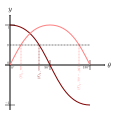
\includegraphics[width = 0.5\textwidth]{dont_use_sine_for_angles}
} 
\end{tabular}

{\bf Examples:}
\begin{itemize}
%%%%
\item If \(B = 45\text{m}\), \(C = 23\text{m}\), and \(\theta_A = 55^\circ\), then 
	\begin{itemize}
	\item[\textasteriskcentered] \(A = \sqrt{B^2 + C^2 - 2BC\cos\theta_A} \approx 36.9689\text{m}\)
	\item[\textasteriskcentered] \(\theta_B = \cos^{-1}\left(\frac{A^2 + C^2 - B^2}{2AC}\right) \approx \cos^{-1}\left(\frac{-129.300\text{m}^2}{1700.57\text{m}^2}\right) \approx 94.3606^\circ\)
	\item[\textasteriskcentered] \(\theta_C = \cos^{-1}\left(\frac{A^2 + B^2 - C^2}{2AB}\right) \approx \cos^{-1}\left(\frac{2862.70\text{m}^2}{3327.20\text{m}^2}\right) \approx 30.6392^\circ\) (note that we could have instead computed \(\theta_C = 180^\circ - \theta_A - \theta_B \approx 30.6394^\circ\). The small difference is due to round-off error.)
	\item[\textasteriskcentered] In summary, \(\theta_A = 55^\circ\), \(\theta_B \approx 94.3606^\circ\), \(\theta_C \approx 30.6392^\circ\), \(A \approx 36.9689\text{m}\), \(B = 45\text{m}\), and \(C = 23\text{m}\).
	\end{itemize}
\end{itemize}


\subsubsection*{Scenario: The given angle is not between the two given sides}

In this scenario, we will be forced to use the sine law to compute angles. Assume that sides \(A\), \(B\) and angle \(\theta_A\) are given. To find \(\theta_B\), the sine law gives \(\frac{A}{\sin\theta_A} = \frac{B}{\sin\theta_B}\) so hence \(\sin\theta_B = \frac{B\sin\theta_A}{A}\). As previously noted, since \(\theta_B\) is confined to the range \([0^\circ, 180^\circ]\) instead of \([0^\circ, 90^\circ]\), there are two possible values of \(\theta_B\): an acute angle \(\theta_B = \sin^{-1}\left(\frac{B\sin\theta_A}{A}\right)\) and an obtuse angle \(\theta_B = 180^\circ - \sin^{-1}\left(\frac{B\sin\theta_A}{A}\right)\). Despite there being apparently two solutions, the obtuse solution for \(\theta_B\) is not possible if the calculated angle for \(\theta_C = 180^\circ - \theta_A - \theta_B\) ends up being negative. 

Once all angles are known, the sine or cosine law can be used to compute the final side length, in this case \(C\).

In the image below, a scenario is presented where knowledge of \(A\), \(B\), and \(\theta_A\) yields two possible triangles. Both values of \(\theta_B\), namely an acute angle of \(\theta_B = \sin^{-1}\left(\frac{B\sin\theta_A}{A}\right)\), and an obtuse angle of \(\theta_B = 180^\circ - \sin^{-1}\left(\frac{B\sin\theta_A}{A}\right)\), yield positive values of \(\theta_C = 180^\circ - \theta_A - \theta_B\) so both triangles are possible. 

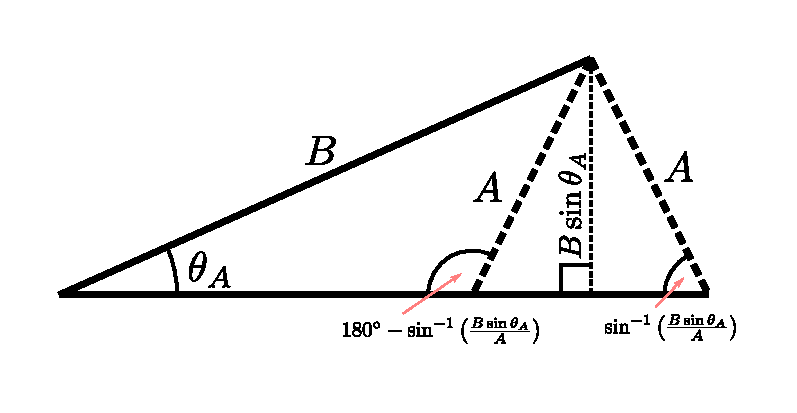
\includegraphics[scale = 1.0]{side_side_angle}

In the image below, a scenario is presented where knowledge of \(A\), \(B\), and \(\theta_A\) yields only one possible triangle. The acute value of \(\theta_B = \sin^{-1}\left(\frac{B\sin\theta_A}{A}\right)\) yields the only positive value of \(\theta_C\), and hence the only valid triangle. The obtuse angle of \(\theta_B = 180^\circ - \sin^{-1}\left(\frac{B\sin\theta_A}{A}\right)\) yields a negative value of \(\theta_C\).

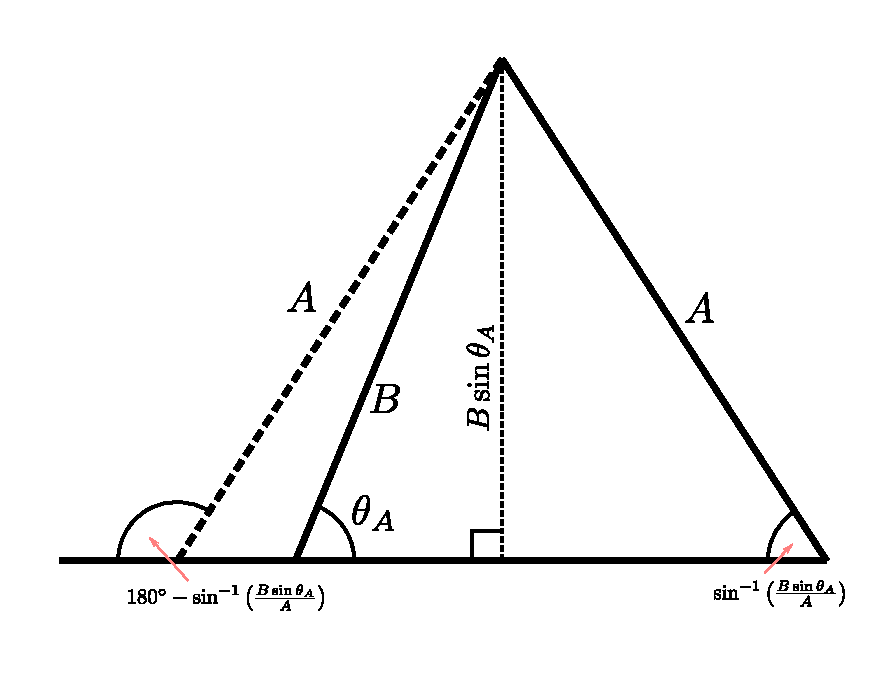
\includegraphics[scale = 1.0]{side_side_angle_2}

{\bf Examples:}
\begin{itemize}
%%%%
\item If \(C = 40\text{m}\), \(A = 69\text{m}\), and \(\theta_C = 26^\circ\), then 
	\begin{itemize}
	\item[\textasteriskcentered] The sine law gives \(\frac{A}{\sin\theta_A} = \frac{C}{\sin\theta_C}\) so \(\sin\theta_A = \frac{A\sin\theta_C}{C} = \frac{(69\text{m})\sin 26^\circ}{40\text{m}} \approx 0.756190\)
	\item[\textasteriskcentered] The two possible values for \(\theta_A\) are \(\theta_A \approx \sin^{-1}(0.756190) \approx 49.1295^\circ\) and \(\theta_A \approx 180^\circ - \sin^{-1}(0.756190) \approx 130.871^\circ\)
	\item[\textasteriskcentered] If \(\theta_A \approx 49.1295^\circ\), then \(\theta_B = 180^\circ - \theta_A - \theta_C \approx 104.871^\circ\) 
	\item[\textasteriskcentered] If \(\theta_A \approx 130.871^\circ\), then \(\theta_B = 180^\circ - \theta_A - \theta_C \approx 23.1290^\circ\) 
	\item[\textasteriskcentered] Both sets of \(\theta_A\), \(\theta_B\), and \(\theta_C\) are valid, so both triangles are valid.
	\item[\textasteriskcentered] Choosing the cosine law to compute \(B\) gives \(B = \sqrt{A^2 + C^2 - 2AC\cos\theta_B} \approx 88.1911\text{m}\) for \(\theta_B \approx 104.871^\circ\) and \(B \approx 35.8425\text{m}\) for \(\theta_B \approx 23.1290^\circ\). Note that we could have also used the sine law to compute \(B = \frac{C\sin\theta_B}{\sin\theta_C} \approx 88.1907\text{m}\) and \(B \approx 35.8420\text{m}\) 
	\item[\textasteriskcentered] In summary, the two triangles are: 
		\begin{itemize}
		\item \(\theta_A \approx 49.1295^\circ\), \(\theta_B \approx 104.871^\circ\), \(\theta_C = 26^\circ\), \(A = 69\text{m}\), \(B \approx 88.1911\text{m}\), and \(C = 40\text{m}\)
		\item \(\theta_A \approx 130.871^\circ\), \(\theta_B \approx 23.1290^\circ\), \(\theta_C = 26^\circ\), \(A = 69\text{m}\), \(B \approx 35.8425\text{m}\), and \(C = 40\text{m}\)
		\end{itemize}
	\end{itemize}
%%%%
\item If \(C = 90\text{m}\), \(A = 69\text{m}\), and \(\theta_C = 26^\circ\), then 
	\begin{itemize}
	\item[\textasteriskcentered] The sine law gives \(\frac{A}{\sin\theta_A} = \frac{C}{\sin\theta_C}\) so \(\sin\theta_A = \frac{A\sin\theta_C}{C} = \frac{(69\text{m})\sin 26^\circ}{90\text{m}} \approx 0.336085\)
	\item[\textasteriskcentered] The two possible values for \(\theta_A\) are \(\theta_A \approx \sin^{-1}(0.336085) \approx 19.6385^\circ\) and \(\theta_A \approx 180^\circ - \sin^{-1}(0.336085) \approx 160.361^\circ\)
	\item[\textasteriskcentered] If \(\theta_A \approx 19.6385^\circ\), then \(\theta_B = 180^\circ - \theta_A - \theta_C \approx 134.362^\circ\) 
	\item[\textasteriskcentered] If \(\theta_A \approx 160.361^\circ\), then \(\theta_B = 180^\circ - \theta_A - \theta_C \approx -6.36100^\circ\). Since \(\theta_B < 0\) for \(\theta_A \approx 160.361^\circ\), \(\theta_A \approx 160.361^\circ\) is not a valid solution.  
	\item[\textasteriskcentered] Choosing the cosine law to compute \(B\) gives \(B = \sqrt{A^2 + C^2 - 2AC\cos\theta_B} \approx 146.782\text{m}\). Note that we could have also used the sine law to compute \(B = \frac{C\sin\theta_B}{\sin\theta_C} \approx 146.780\text{m}\)
	\item[\textasteriskcentered] In summary, \(\theta_A \approx 19.6385^\circ\), \(\theta_B \approx 134.362^\circ\), \(\theta_C = 26^\circ\), \(A = 69\text{m}\), \(B \approx 146.782\text{m}\), and \(C = 90\text{m}\)
	\end{itemize}
%%%%
\item If \(B = 7.8\text{m}\), \(C = 6.124\text{m}\), and \(\theta_B = 130^\circ\), then 
	\begin{itemize}
	\item[\textasteriskcentered] The sine law gives \(\frac{B}{\sin\theta_B} = \frac{C}{\sin\theta_C}\) so \(\sin\theta_C = \frac{C\sin\theta_B}{B} = \frac{(6.124\text{m})\sin 130^\circ}{7.8\text{m}} \approx 0.601443\) 
	\item[\textasteriskcentered] The two possible values for \(\theta_C \approx \sin^{-1}(0.601443) \approx 36.9733^\circ\) and \(\theta_C \approx 180^\circ - \sin^{-1}(0.601443) \approx 143.027^\circ\)
	\item[\textasteriskcentered] If \(\theta_C \approx 36.9733^\circ\), then \(\theta_A = 180^\circ - \theta_B - \theta_C \approx 13.0267^\circ\)
	\item[\textasteriskcentered] If \(\theta_C \approx 143.027^\circ\), then \(\theta_A = 180^\circ - \theta_B - \theta_C \approx -93.0270^\circ\). Since \(\theta_A < 0\) for \(\theta_C \approx 143.027^\circ\), \(\theta_C \approx 143.027^\circ\) is not a valid solution.  
	\item[\textasteriskcentered] Choosing the cosine law to compute \(A\) gives \(A = \sqrt{B^2 + C^2 - 2BC\cos\theta_A} \approx 2.29511\text{m}\). Note that we could have also used the sine law to compute \(A = \frac{B\sin\theta_A}{\sin\theta_B} \approx 2.29511\text{m}\)
	\item[\textasteriskcentered] In summary, \(\theta_A \approx 13.0267^\circ\), \(\theta_B = 130^\circ\), \(\theta_C \approx 36.9733^\circ\), \(A \approx 2.29511\text{m}\), \(B = 7.8\text{m}\), and \(C = 6.124\text{m}\)
	\end{itemize}
\end{itemize}




\section*{Error checking}

As seen above, the process of solving a triangle is complicated, and hard-to-find mistakes can be made at any point during the process. Given side lengths \(A\), \(B\), and \(C\); and angles \(\theta_A\), \(\theta_B\), and \(\theta_C\); we desire a way of checking that the sides and angles describe a valid triangle. We desire these tests so that we may catch errors in our work. 

Firstly, the angles in a triangle must sum to \(180^\circ\). Hence \(\theta_A + \theta_B + \theta_C\) must be very close to \(180^\circ\) (we use very close instead of exact because round-off error will invariably introduce errors). 

Next, the length of the altitude that descends from the vertex that contains \(\theta_C\) and is perpendicular to side \(C\) can be computed by either \(A\sin\theta_B\) or \(B\sin\theta_A\). The {\bf relative} error between these two computed lengths must be very small so \(\frac{A\sin\theta_B}{B\sin\theta_A}\) must be very close to \(1\). By similar argument, \(\frac{A\sin\theta_C}{C\sin\theta_A}\) and \(\frac{B\sin\theta_C}{C\sin\theta_B}\) must also be very close to \(1\). 

In summary, the battery of tests that our angles and side lengths must pass are:
\begin{itemize}
\item \(\theta_A + \theta_B + \theta_C \approx 180^\circ\)
\item \(\frac{A\sin\theta_B}{B\sin\theta_A} \approx 1\)
\item \(\frac{A\sin\theta_C}{C\sin\theta_A} \approx 1\)
\item \(\frac{B\sin\theta_C}{C\sin\theta_B} \approx 1\) (this last test will actually hold if the previous two tests hold, and can be omitted for speed)
\end{itemize} 



\end{document}










